% Provenance (never printed): cycle 3 "La planete Terre" and geography
% (weather and climate; reading a climate chart; the great climate zones of
% the world, hot, temperate and cold); see sources/book1/PROVENANCE.md.
% Book 1, grade 5, chapter 2.
\chapter{Cuaca dan Iklim}\label{ch:g5:weather-and-climate}

Pada minggu kedua bulan Januari, dua kartu pos tiba di sekolah. Kartu
pertama, dari sepupu Lena, bergambar anak-anak yang membuat istana \omterm{def:g3:stones-pebbles-sand:sand}{pasir} di
pantai yang cerah di bawah pohon-pohon kelapa. Kartu kedua, dari nenek Tom,
bergambar anak-anak yang membuat boneka salju di kebun yang bersalju.
``Bagaimana bisa musim panas dan musim dingin terjadi pada minggu yang
sama?'' tanya Tom.

Yang begitu berbeda di antara kedua tempat itu bukanlah \omterm{def:g1:watching-the-weather:weather}{cuaca} pada satu
hari. Yang berbeda adalah \omterm{def:g1:watching-the-weather:weather}{cuaca} yang mereka alami, dari tahun ke tahun:
\omterm{def:g5:weather-and-climate:climate}{iklimnya}.

\begin{omfigure}
\begin{minipage}[b]{0.48\linewidth}\centering

\includegraphics[width=\linewidth]{images/book1/ai/g5-beach-postcard.jpg}
\end{minipage}\hfill
\begin{minipage}[b]{0.48\linewidth}\centering

\includegraphics[width=\linewidth]{images/book1/ai/g5-snowman-postcard.jpg}
\end{minipage}

{\small Dua kartu pos dari minggu yang sama di bulan Januari: pantai yang
cerah dan kebun yang bersalju.}
\end{omfigure}

\begin{recall}
\omterm{def:g1:watching-the-weather:weather}{Cuaca} adalah keadaan udara di suatu tempat pada suatu waktu: cerah,
berawan, \omterm{def:g4:clouds-rain-snow:precipitation}{hujan}, bersalju, berangin (\cref{ch:g1:watching-the-weather}).
Termometer mengukur suhu udara, dalam derajat Celsius; \omterm{def:g4:clouds-rain-snow:rain-gauge}{penakar hujan}
mengukur \omterm{def:g4:clouds-rain-snow:precipitation}{hujan}, dalam milimeter (\cref{ch:g4:clouds-rain-snow}).
\omterm{def:g3:continents-and-oceans:equator}{Khatulistiwa} melingkari bagian tengah \omterm{def:g3:continents-and-oceans:globe}{bola dunia}, di pertengahan antara
\omterm{def:g3:continents-and-oceans:poles}{Kutub Utara} dan \omterm{def:g3:continents-and-oceans:poles}{Kutub Selatan} (\cref{ch:g3:continents-and-oceans}). Buku
fisika telah menunjukkan bahwa Bumi mengelilingi Matahari dalam satu tahun,
dan bahwa musim-musimnya berasal dari kemiringan sumbunya: pada musim
panas, Matahari naik lebih tinggi di langit dan siang hari lebih panjang.
\end{recall}

\section{Cuaca adalah hari ini, iklim adalah yang biasa}

\omterm{def:g1:watching-the-weather:weather}{Cuaca} berubah dari hari ke hari, bahkan dari jam ke jam. \omterm{def:g5:weather-and-climate:climate}{Iklim} adalah hal
yang lain.

\begin{definition}[Iklim]\label{def:g5:weather-and-climate:climate}
Yang disebut \emph{iklim}\index{iklim} suatu tempat adalah \omterm{def:g1:watching-the-weather:weather}{cuaca} yang
biasanya terjadi di sana, bulan demi bulan, selama bertahun-tahun: seberapa
hangat atau dingin, seberapa basah atau kering setiap musimnya. Para ahli
\omterm{def:g1:watching-the-weather:weather}{cuaca} menghitungnya dengan merata-ratakan hasil pengukuran selama 30 tahun.
% ledger: wmo:normal-30yr
\end{definition}

``Pagi ini \omterm{def:g4:clouds-rain-snow:precipitation}{hujan} turun'' adalah kalimat tentang \omterm{def:g1:watching-the-weather:weather}{cuaca}. ``Di sini banyak
\omterm{def:g4:clouds-rain-snow:precipitation}{hujan} pada musim gugur'' adalah kalimat tentang \omterm{def:g5:weather-and-climate:climate}{iklim}. Satu hari yang
dingin di musim panas tidak mengubah \omterm{def:g5:weather-and-climate:climate}{iklim}; itu hanyalah \omterm{def:g1:watching-the-weather:weather}{cuaca} yang tidak
biasa.

Para ahli \omterm{def:g1:watching-the-weather:weather}{cuaca} di seluruh dunia memakai aturan yang sama: mereka
merata-ratakan hasil pengukuran selama 30 tahun. Rata-rata yang dipakai
sekarang adalah rata-rata tahun 1991 sampai 2020.
% ledger: wmo:normal-30yr

\section{Diagram iklim}

Untuk menunjukkan \omterm{def:g5:weather-and-climate:climate}{iklim} suatu tempat dalam satu gambar, kita membuat
sebuah diagram.

\begin{definition}[Diagram iklim]\label{def:g5:weather-and-climate:climate-chart}
Yang disebut \emph{diagram iklim}\index{diagram iklim} menunjukkan, untuk
setiap bulan dalam setahun, suhu rata-rata suatu tempat (sebuah kurva) dan
jumlah rata-rata \omterm{def:g4:clouds-rain-snow:precipitation}{hujan} dan \omterm{def:g4:clouds-rain-snow:precipitation}{salju} yang turun di sana (batang-batang, dalam
milimeter air).
\end{definition}

\begin{omfigure}
\begin{tikzpicture}
  \begin{axis}[name=pax, width=0.55\linewidth, height=5.6cm, ymin=0, ymax=400,
      axis y line*=right, axis x line=none, ybar, bar width=7pt,
      ytick={0,100,...,400}, ylabel={hujan (mm)}, xmin=0.4, xmax=12.6,
      tick label style={font=\scriptsize}, label style={font=\scriptsize},
      ylabel style={blue!60!black}]
    \addplot[fill=blue!40, draw=blue!60!black]
      table[x=month, y=prcp_mm] {figdata/out/grade-5-climate_charts-seattle.dat};
  \end{axis}
  \begin{axis}[width=0.55\linewidth, height=5.6cm, ymin=-30, ymax=40,
      axis y line*=left, axis x line*=bottom, xmin=0.4, xmax=12.6,
      xtick={1,...,12}, xticklabels={J,F,M,A,M,J,J,A,S,O,N,D},
      ytick={-30,-20,...,40}, ylabel={suhu ($^\circ$C)},
      tick label style={font=\scriptsize}, label style={font=\scriptsize},
      ylabel style={red!70!black}]
    \addplot[red!70!black, thick, mark=*, mark size=1.3pt]
      table[x=month, y=tavg_C] {figdata/out/grade-5-climate_charts-seattle.dat};
    \draw[gray!60] (axis cs:0.4,0) -- (axis cs:12.6,0);
    \begin{scope}[every node/.style={circle, draw, fill=white, inner sep=0.8pt,
        font=\scriptsize\bfseries}]
      \node[text=red!70!black, draw=red!70!black] at (axis cs:5.5,27) {1};
      \node[text=blue!60!black, draw=blue!60!black] at (axis cs:7,-19) {2};
    \end{scope}
  \end{axis}
  \node[anchor=north west, font=\scriptsize, align=left, text width=4.2cm]
    at ($(pax.outer north east)+(0.3,-0.1)$) {%
    \textcolor{red!70!black}{\textbf{1} Kurva merah: suhu rata-rata setiap
    bulan, dibaca pada skala kiri.}\par\smallskip
    \textcolor{blue!60!black}{\textbf{2} Batang biru: hujan rata-rata setiap
    bulan, dibaca pada skala kanan.}\par\smallskip
    \textbf{3} Huruf-huruf di bawah diagram: bulan-bulan, Januari sampai
    Desember.};
\end{tikzpicture}

{\small \omterm{def:g5:weather-and-climate:climate-chart}{Diagram iklim} Seattle, sebuah kota di \omterm{def:g1:landscapes-around-us:water}{pesisir} barat Amerika Serikat.
Rata-rata tahun 1991 sampai 2020 (data: NOAA).}
% ledger: data:b1-noaa-normals
\end{omfigure}

\begin{method}[Membaca diagram iklim]\label{met:g5:weather-and-climate:reading}
\begin{enumerate}
  \item Cari bulan yang paling hangat dan yang paling dingin pada kurva
        merah, lalu baca suhunya pada skala kiri. Apakah kurvanya datar
        (suhunya sama sepanjang tahun) atau naik dan turun (ada musim hangat
        dan musim dingin)? Apakah kurvanya turun di bawah 0~$^\circ$C
        (membeku)?
  \item Cari bulan yang paling basah dan yang paling kering di antara
        batang-batang biru, lalu baca nilainya pada skala kanan. Apakah
        batangnya tinggi atau pendek? Apakah ada musim kemarau?
  \item Satukan semuanya dalam satu kalimat: ``panas dan kering sepanjang
        tahun'', ``sejuk dan basah, dengan musim panas yang kering''{\ldots}
\end{enumerate}
\end{method}

\begin{example}[Seattle]\label{ex:g5:weather-and-climate:seattle}
Di Seattle, bulan yang paling hangat adalah Agustus (kira-kira
20~$^\circ$C) dan yang paling dingin adalah Desember (kira-kira
6~$^\circ$C): kurvanya naik dan turun, tetapi tidak pernah turun di bawah
titik beku. Batang yang paling tinggi adalah batang November (kira-kira
160~mm), yang paling pendek batang Juli (kira-kira 15~mm). Dalam satu
kalimat: musim dingin yang sejuk, musim panas yang segar, basah pada musim
gugur dan musim dingin, agak kering pada musim panas. Dalam satu tahun
penuh, kira-kira 1\,000~milimeter \omterm{def:g4:clouds-rain-snow:precipitation}{hujan} turun: satu meter air.
% ledger: data:b1-noaa-normals
\end{example}

\section{Empat iklim}

Berikut ini \omterm{def:g5:weather-and-climate:climate-chart}{diagram iklim} empat kota di Amerika Serikat yang letaknya
berjauhan: Phoenix, di \omterm{def:g5:weather-and-climate:desert}{gurun} Arizona; Hilo, di Pulau Hawaii di tengah
\omterm{def:g2:water-on-earth:ocean}{Samudra} Pasifik; Seattle, di \omterm{def:g1:landscapes-around-us:water}{pesisir} barat; dan Utqiaġvik, di ujung utara
Alaska, di \omterm{def:g1:landscapes-around-us:water}{pesisir} \omterm{def:g2:water-on-earth:ocean}{Samudra} Arktik. Keempat diagram memakai skala yang sama,
sehingga kita dapat membandingkannya sekilas.

\begin{omfigure}
\def\gfivechart#1#2{%
\begin{tikzpicture}
  \begin{axis}[width=0.5\linewidth, height=4.6cm, ymin=0, ymax=400,
      axis y line*=right, axis x line=none, ybar, bar width=4pt,
      ytick={0,100,...,400}, xmin=0.4, xmax=12.6,
      tick label style={font=\tiny}]
    \addplot[fill=blue!40, draw=blue!60!black]
      table[x=month, y=prcp_mm] {figdata/out/grade-5-climate_charts-#1.dat};
  \end{axis}
  \begin{axis}[width=0.5\linewidth, height=4.6cm, ymin=-30, ymax=40,
      axis y line*=left, axis x line*=bottom, xmin=0.4, xmax=12.6,
      xtick={1,...,12}, xticklabels={J,F,M,A,M,J,J,A,S,O,N,D},
      ytick={-30,-20,...,40}, tick label style={font=\tiny},
      title={#2}, title style={font=\scriptsize\bfseries, yshift=-4pt}]
    \addplot[red!70!black, thick, mark=*, mark size=1pt]
      table[x=month, y=tavg_C] {figdata/out/grade-5-climate_charts-#1.dat};
    \draw[gray!60] (axis cs:0.4,0) -- (axis cs:12.6,0);
  \end{axis}
\end{tikzpicture}}%
\gfivechart{phoenix}{Phoenix: \omterm{def:g5:weather-and-climate:desert}{gurun} panas}\hfill
\gfivechart{hilo}{Hilo: \omterm{def:g5:weather-and-climate:climate}{iklim} \omterm{def:g5:weather-and-climate:rainforest}{hutan hujan}}

\medskip
\gfivechart{seattle}{Seattle: \omterm{def:g5:weather-and-climate:climate}{iklim} sedang}\hfill
\gfivechart{utqiagvik}{Utqiaġvik: \omterm{def:g5:weather-and-climate:climate}{iklim} \omterm{def:g3:continents-and-oceans:poles}{kutub}}

{\small Empat \omterm{def:g5:weather-and-climate:climate-chart}{diagram iklim} dengan skala yang sama: suhu dalam $^\circ$C di
sebelah kiri (kurva merah), \omterm{def:g4:clouds-rain-snow:precipitation}{hujan} dalam milimeter di sebelah kanan (batang
biru). Rata-rata tahun 1991 sampai 2020 (data: NOAA).}
% ledger: data:b1-noaa-normals
\end{omfigure}

\paragraph{Gurun.} Di Phoenix, batang-batangnya begitu pendek sehingga kita
hampir tidak dapat melihatnya: dalam satu tahun penuh, kurang dari
200 milimeter \omterm{def:g4:clouds-rain-snow:precipitation}{hujan} turun. Musim panasnya sangat panas: pada bulan Juli suhu
rata-ratanya 35 derajat.
% ledger: data:b1-noaa-normals

\begin{definition}[Gurun]\label{def:g5:weather-and-climate:desert}
Yang disebut \emph{gurun}\index{gurun} adalah tempat yang sangat sedikit
menerima \omterm{def:g4:clouds-rain-snow:precipitation}{hujan}: kurang dari 250 milimeter dalam setahun. Hanya sedikit
tumbuhan yang dapat hidup di sana, dan tanahnya sering kali gundul.
% ledger: usgs:arid-250mm
\end{definition}

\omterm{def:g5:weather-and-climate:desert}{Gurun} tidak selalu panas. Lihatlah Utqiaġvik: kurang dari 150 milimeter
\omterm{def:g4:clouds-rain-snow:precipitation}{hujan} turun di sana dalam setahun, bahkan lebih sedikit daripada di
Phoenix: tempat itu adalah \omterm{def:g5:weather-and-climate:desert}{gurun} dingin. \omterm{def:g5:weather-and-climate:desert}{Gurun} bisa panas atau dingin.
% ledger: data:b1-noaa-normals, usgs:arid-250mm

\paragraph{Hutan hujan.} Hilo adalah kebalikan dari Phoenix. Batang-batangnya
adalah yang paling tinggi di antara keempat diagram: lebih dari
3\,000 milimeter \omterm{def:g4:clouds-rain-snow:precipitation}{hujan} turun dalam setahun, dan setiap bulannya basah.
Kurva merahnya pun hampir datar: antara 22 dan 25 derajat sepanjang tahun.
Di sana sama sekali tidak ada musim dingin.
% ledger: data:b1-noaa-normals

\begin{definition}[Hutan hujan]\label{def:g5:weather-and-climate:rainforest}
Yang disebut \emph{hutan hujan}\index{hutan hujan} adalah hutan lebat dengan
pohon-pohon yang sangat tinggi, yang tumbuh di tempat yang hangat dan basah
sepanjang tahun, dengan \omterm{def:g4:clouds-rain-snow:precipitation}{hujan} lebat setiap bulan. Sebagian besar hutan \omterm{def:g4:clouds-rain-snow:precipitation}{hujan}
terletak di dekat \omterm{def:g3:continents-and-oceans:equator}{khatulistiwa}.
\end{definition}

\begin{omfigure}
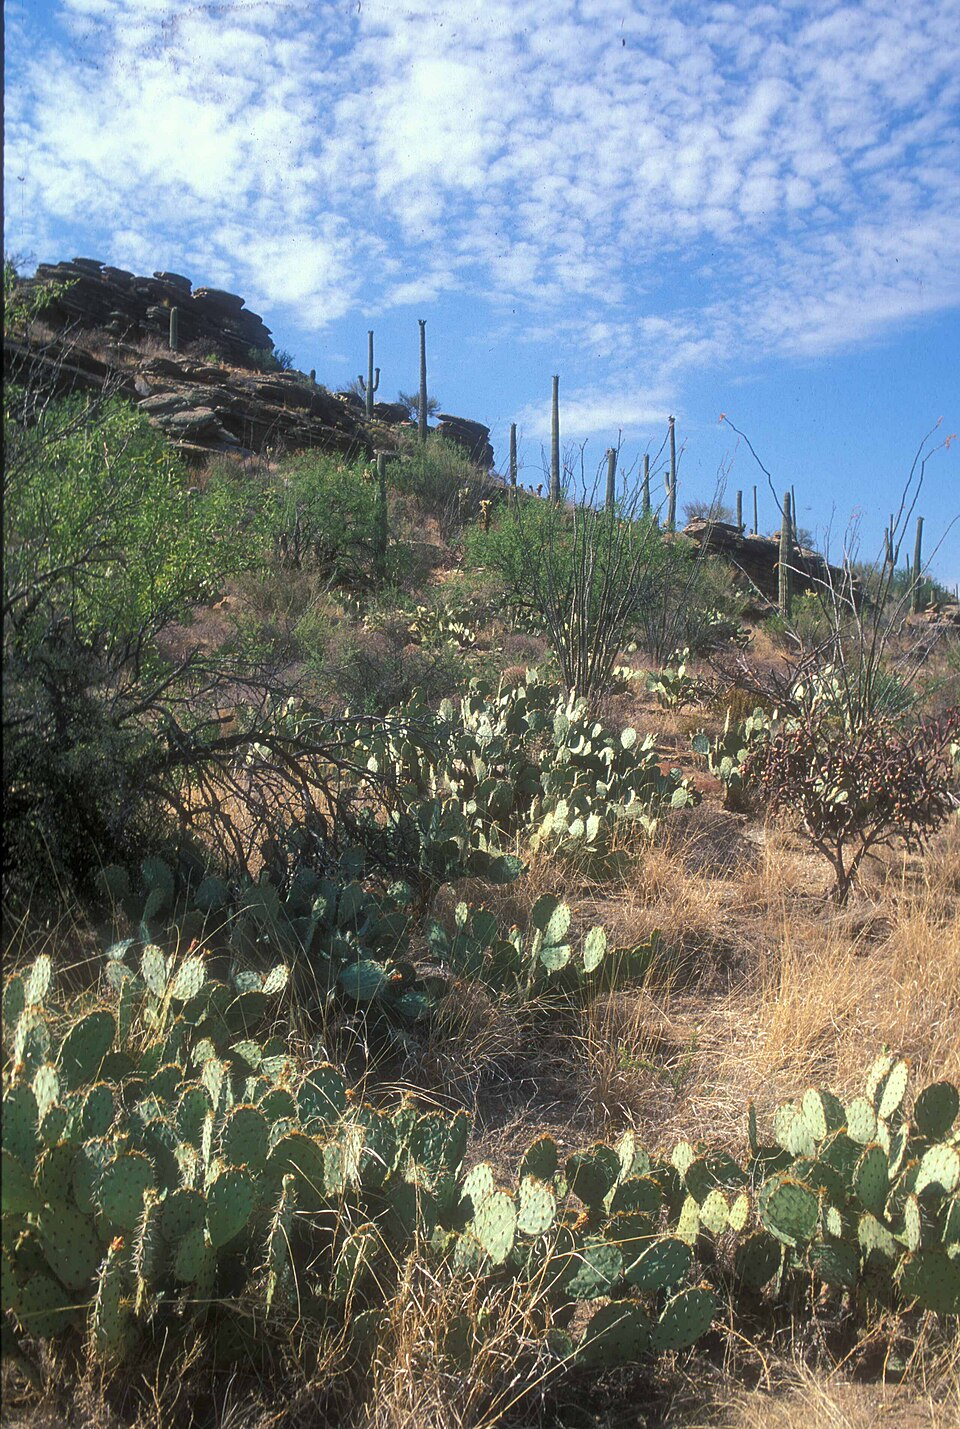
\includegraphics[height=3.6cm]{images/book1/g5-sonoran-desert.jpg}\quad
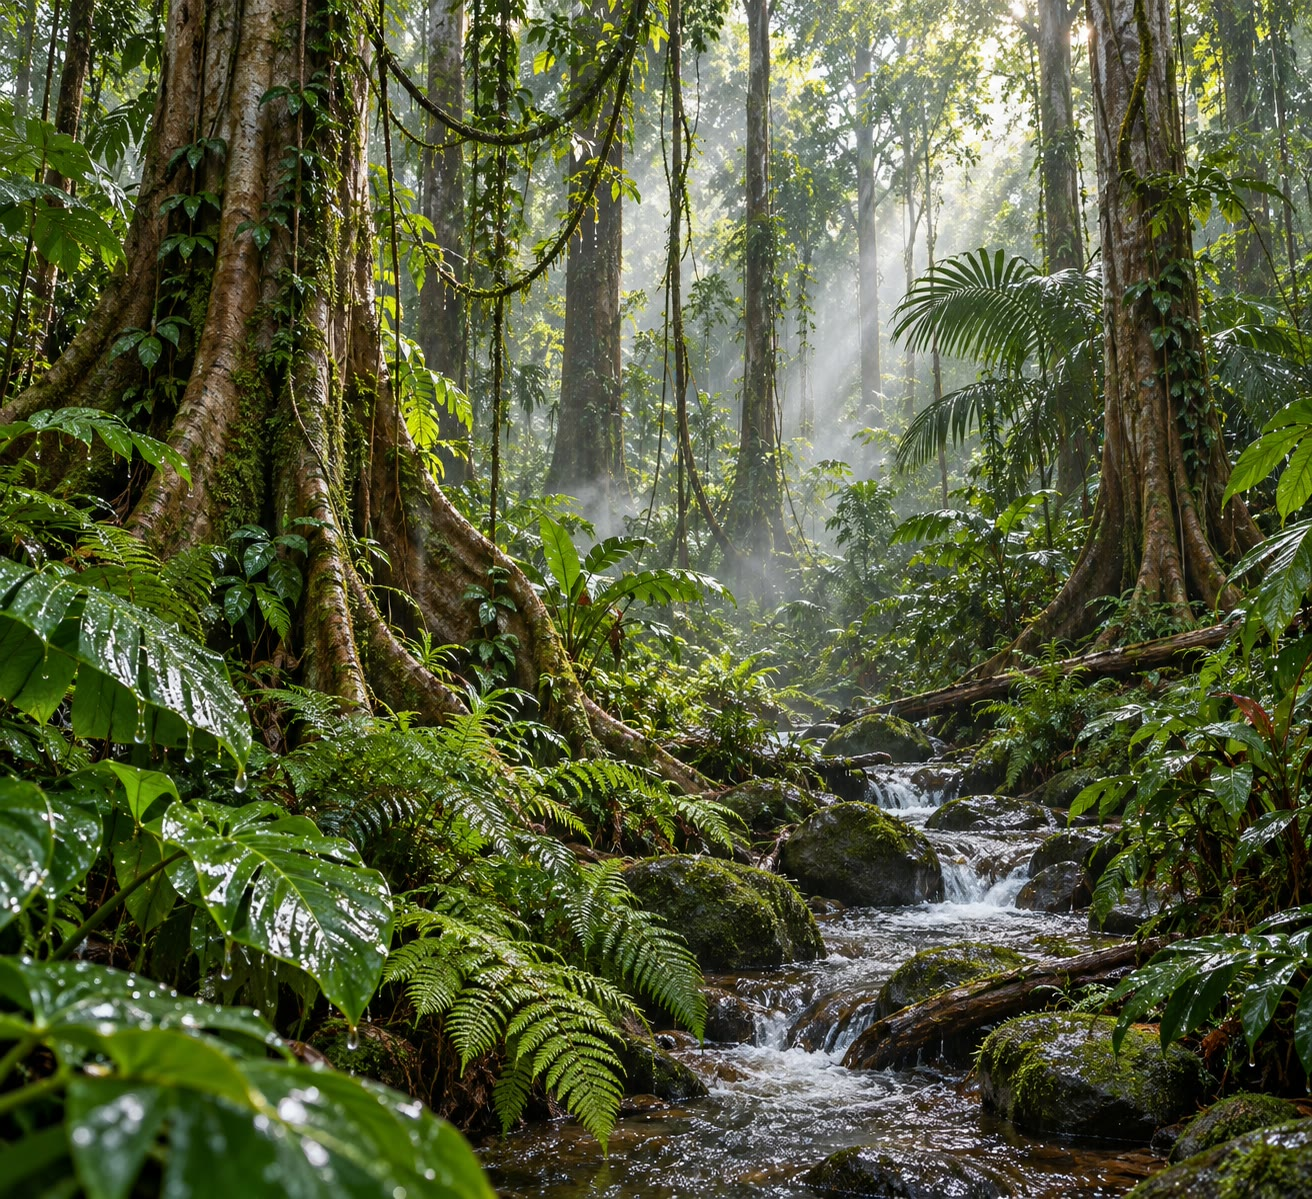
\includegraphics[height=3.6cm]{images/book1/ai/g5-rainforest.jpg}\quad
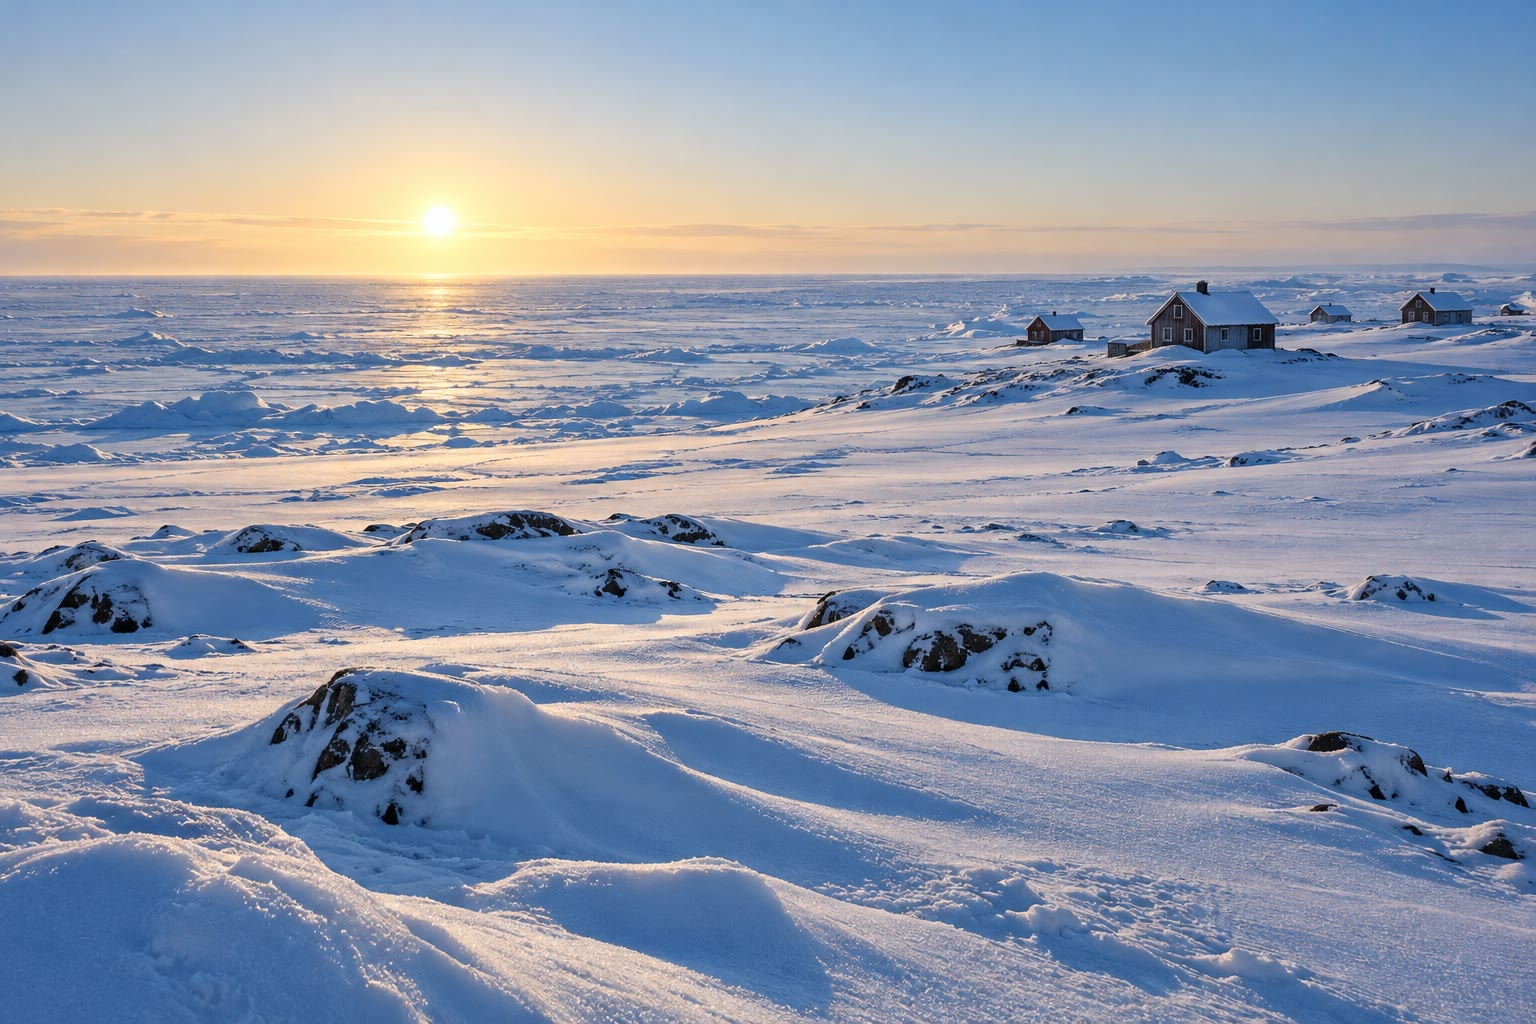
\includegraphics[height=3.6cm]{images/book1/ai/g5-polar-tundra.jpg}

{\small Tiga \omterm{def:g5:weather-and-climate:climate}{iklim} yang ekstrem. Kiri: \omterm{def:g5:weather-and-climate:desert}{Gurun} Sonora di Arizona, \omterm{def:g5:weather-and-climate:desert}{gurun}
tempat Phoenix berada, dengan kaktus saguaro yang tinggi dan kaktus pir
berduri, yang menyimpan air di dalam batangnya yang tebal (foto: U.S.
National Park Service, Saguaro National Park, domain publik). Tengah: di
dalam \omterm{def:g5:weather-and-climate:rainforest}{hutan hujan} setelah \omterm{def:g4:clouds-rain-snow:precipitation}{hujan} sebentar. Kanan: \omterm{def:g1:landscapes-around-us:water}{pesisir} \omterm{def:g3:continents-and-oceans:poles}{kutub} pada musim
dingin, dengan \omterm{def:g2:water-on-earth:ocean}{laut} yang membeku dan Matahari yang rendah pada tengah hari.}
% ledger: nps:sonoran-desert
\end{omfigure}

\paragraph{Iklim sedang.} Seattle berada di antara keduanya: kurvanya naik
pada musim panas dan turun pada musim dingin, tetapi tidak pernah terlalu
jauh; \omterm{def:g4:clouds-rain-snow:precipitation}{hujannya} cukup banyak, terutama pada musim gugur dan musim dingin.
Inilah \omterm{def:g5:weather-and-climate:climate}{iklim} sedang: tidak sangat panas, tidak sangat dingin.

\paragraph{Iklim kutub.} Di Utqiaġvik, kurva merahnya tetap di bawah
0~$^\circ$C selama delapan bulan dalam setahun; pada bulan Februari
rata-ratanya 24 derajat di bawah nol. Bahkan pada bulan Juli, bulan yang
paling hangat, suhunya hanya kira-kira 5 derajat.
% ledger: data:b1-noaa-normals

\section{Zona panas, zona sedang, dan zona dingin}

Mengapa di dekat \omterm{def:g3:continents-and-oceans:equator}{khatulistiwa} udaranya hangat dan di dekat \omterm{def:g3:continents-and-oceans:poles}{kutub} dingin?
Karena Matahari. Di dekat \omterm{def:g3:continents-and-oceans:equator}{khatulistiwa}, Matahari tengah hari berada tinggi
di langit sepanjang tahun: cahayanya jatuh hampir tegak lurus dan
menghangatkan tanah dengan kuat. Di dekat \omterm{def:g3:continents-and-oceans:poles}{kutub}, Matahari selalu rendah:
cahayanya datang miring, tersebar di atas daerah yang luas, dan hanya
sedikit menghangatkan. Pada musim dingin di sana, Matahari bahkan mungkin
tidak terbit sama sekali.

Dua pasang garis yang melingkari \omterm{def:g3:continents-and-oceans:globe}{bola dunia} membagi Bumi menjadi \omterm{def:g5:weather-and-climate:climate-zone}{zona-zona
iklim}.

\begin{definition}[Garis balik dan lingkaran kutub]\label{def:g5:weather-and-climate:tropics}
Yang disebut kedua \emph{garis balik}\index{garis balik} adalah garis-garis
yang melingkari \omterm{def:g3:continents-and-oceans:globe}{bola dunia}, satu di utara dan satu di selatan \omterm{def:g3:continents-and-oceans:equator}{khatulistiwa},
yang menandai seberapa jauh dari \omterm{def:g3:continents-and-oceans:equator}{khatulistiwa} Matahari tengah hari dapat
berada tepat di atas kepala: Garis Balik Utara di utara, Garis Balik
Selatan di selatan. Yang disebut kedua \emph{lingkaran
kutub}\index{lingkaran kutub} adalah garis-garis yang melingkari \omterm{def:g3:continents-and-oceans:globe}{bola dunia},
di dekat \omterm{def:g3:continents-and-oceans:poles}{kutub}, yang di luarnya, pada pertengahan musim dingin, Matahari
tidak terbit setidaknya selama satu hari, dan pada pertengahan musim panas
Matahari tidak terbenam: Lingkaran Arktik di utara, Lingkaran Antarktik di
selatan.
\end{definition}

Kemiringan sumbu Bumi menentukan letak garis-garis ini.

\begin{definition}[Zona iklim]\label{def:g5:weather-and-climate:climate-zone}
Bumi terbagi menjadi tiga jenis \emph{zona iklim}\index{zona iklim}: \emph{zona panas}, di antara kedua \omterm{def:g5:weather-and-climate:tropics}{garis balik}, di sekitar \omterm{def:g3:continents-and-oceans:equator}{khatulistiwa};
dua \emph{zona sedang}, di antara sebuah \omterm{def:g5:weather-and-climate:tropics}{garis balik} dan sebuah \omterm{def:g5:weather-and-climate:tropics}{lingkaran
kutub}, tempat musim panas dan musim dingin berbeda; dan dua \emph{zona
dingin}, di luar \omterm{def:g5:weather-and-climate:tropics}{lingkaran kutub}, di sekitar \omterm{def:g3:continents-and-oceans:poles}{kutub}.
\end{definition}

\begin{omfigure}
\begin{tikzpicture}
\begin{axis}[ommap, width=\linewidth, xtick=\empty, ytick=\empty, grid=none,
    axis background/.style={fill=white}, clip=true]
  \addplot[fill=orange!35, draw=none] table {figdata/out/grade-5-climate_zones-hot.dat};
  \addplot[fill=green!20, draw=none] table {figdata/out/grade-5-climate_zones-temperate.dat};
  \addplot[fill=cyan!20, draw=none] table {figdata/out/grade-5-climate_zones-cold.dat};
  \addplot[fill=black!25, fill opacity=0.8, draw=black!60, line width=0.2pt]
    table {figdata/out/shared-geo-land.dat};
  \addplot[black!70, dashed, line width=0.5pt] table {figdata/out/grade-5-climate_zones-lines.dat};
  \draw[black!70, line width=0.6pt] (axis cs:-180,0) -- (axis cs:180,0);
  \addplot[only marks, mark=*, mark size=1.8pt, red!80!black]
    table[x=lon, y=lat] {figdata/out/grade-5-climate_zones-stations.dat};
  \begin{scope}[every node/.style={font=\scriptsize, fill=white, fill opacity=0.75,
      text opacity=1, inner sep=1pt}]
    \node[anchor=west] at (axis cs:-107,33.4) {Phoenix};
    \node[anchor=east] at (axis cs:-158,19.7) {Hilo};
    \node[anchor=west] at (axis cs:-117,47.4) {Seattle};
    \node[anchor=west] at (axis cs:-151,73.5) {Utqiaġvik};
  \end{scope}
  \begin{scope}[every node/.style={font=\scriptsize\bfseries, align=center,
      fill=white, fill opacity=0.7, text opacity=1, inner sep=1pt}]
    \node at (axis cs:-5,83) {zona dingin};
    \node at (axis cs:-40,40) {zona sedang};
    \node at (axis cs:-25,-8) {zona panas};
    \node at (axis cs:95,-45) {zona sedang};
    \node at (axis cs:-60,-80) {zona dingin};
  \end{scope}
\end{axis}
\end{tikzpicture}

{\small \omterm{def:g5:weather-and-climate:climate-zone}{Zona-zona iklim}. Dari atas ke bawah, garis-garis putus-putus itu
adalah Lingkaran Arktik, \omterm{def:g5:weather-and-climate:tropics}{Garis Balik} Utara, \omterm{def:g5:weather-and-climate:tropics}{Garis Balik} Selatan, dan
Lingkaran Antarktik; garis yang tidak terputus adalah \omterm{def:g3:continents-and-oceans:equator}{khatulistiwa}.
Titik-titik merah adalah keempat kota pada \omterm{def:g5:weather-and-climate:climate-chart}{diagram iklim} di atas.}
% ledger: earth:obliquity, data:b1-noaa-normals
\end{omfigure}

Zona-zona itu memberikan gambaran awal yang kasar. Di dalam setiap zona,
banyak hal lain yang mengubah \omterm{def:g5:weather-and-climate:climate}{iklim}: seberapa jauh suatu tempat dari \omterm{def:g2:water-on-earth:ocean}{laut},
seberapa tinggi letaknya, dari mana anginnya datang. Kamu akan mempelajarinya
di kelas-kelas berikutnya.

\begin{remark}[Phoenix dan zona-zona]\label{rem:g5:weather-and-climate:phoenix}
Pada \omterm{def:g2:drawing-to-map:map}{peta} zona, Phoenix terletak sedikit di utara \omterm{def:g5:weather-and-climate:tropics}{Garis Balik} Utara, di zona
sedang, tetapi kota itu adalah \omterm{def:g5:weather-and-climate:desert}{gurun} panas. Zona-zona itu hanyalah gambaran
awal yang kasar: banyak \omterm{def:g5:weather-and-climate:desert}{gurun} panas yang besar terletak di dekat \omterm{def:g5:weather-and-climate:tropics}{garis
balik}, di tepi zona panas, dan kamu akan mengetahui sebabnya dalam
\cref{ch:g8:winds-global-circulation}.
\end{remark}

\section{Latihan}

\begin{exercise}[$\star$]\label{exo:g5:weather-and-climate:1}
\omterm{def:g1:watching-the-weather:weather}{Cuaca} atau \omterm{def:g5:weather-and-climate:climate}{iklim}?
\begin{enumerate}
  \item[(a)] Pagi ini \omterm{def:g4:clouds-rain-snow:precipitation}{salju} turun di Utqiaġvik.
  \item[(b)] Di Phoenix, musim panasnya sangat panas dan kering.
  \item[(c)] Kemarin sore angin kencang bertiup di Seattle.
  \item[(d)] Di Hilo, banyak \omterm{def:g4:clouds-rain-snow:precipitation}{hujan} turun setiap bulan sepanjang tahun.
\end{enumerate}
\end{exercise}

\begin{exercise}[$\star$]\label{exo:g5:weather-and-climate:2}
Apa yang dimaksud dengan \omterm{def:g5:weather-and-climate:climate}{iklim} suatu tempat? Selama berapa tahun para ahli
\omterm{def:g1:watching-the-weather:weather}{cuaca} merata-ratakan hasil pengukurannya untuk menggambarkan \omterm{def:g5:weather-and-climate:climate}{iklim} itu?
\end{exercise}

\begin{exercise}[$\star$]\label{exo:g5:weather-and-climate:3}
Pada \omterm{def:g5:weather-and-climate:climate-chart}{diagram iklim} Seattle, bulan apa yang paling dingin? Bulan apa yang
paling basah? Apakah suhunya pernah turun di bawah 0~$^\circ$C?
\end{exercise}

\begin{exercise}[$\star$]\label{exo:g5:weather-and-climate:4}
Pada \omterm{def:g5:weather-and-climate:climate-chart}{diagram iklim} Utqiaġvik, bulan apa yang paling hangat? Adakah bulan
yang suhunya lebih dari 10~$^\circ$C?
\end{exercise}

\begin{exercise}[$\star$]\label{exo:g5:weather-and-climate:5}
Di \omterm{def:g5:weather-and-climate:climate-zone}{zona iklim} manakah setiap tempat berikut: \omterm{def:g3:continents-and-oceans:equator}{khatulistiwa}; \omterm{def:g3:continents-and-oceans:poles}{Kutub Utara};
sebuah tempat di pertengahan antara \omterm{def:g3:continents-and-oceans:equator}{khatulistiwa} dan \omterm{def:g3:continents-and-oceans:poles}{Kutub Selatan}?
\end{exercise}

\begin{exercise}[$\star$]\label{exo:g5:weather-and-climate:6}
Gunakan \omterm{def:g2:drawing-to-map:map}{peta} zona. Di \omterm{def:g5:weather-and-climate:climate-zone}{zona iklim} manakah setiap kota dari keempat kota itu:
Phoenix, Hilo, Seattle, Utqiaġvik?
\end{exercise}

\begin{exercise}[$\star\star$]\label{exo:g5:weather-and-climate:7}
Berikut ini \omterm{def:g4:clouds-rain-snow:precipitation}{hujan} rata-rata setiap bulan di Seattle, dalam milimeter,
dibulatkan ke bilangan bulat:
\begin{center}
\begin{tabular}{|*{12}{c|}}
\hline
J & F & M & A & M & J & J & A & S & O & N & D\\
\hline
147 & 96 & 106 & 81 & 48 & 37 & 15 & 25 & 41 & 99 & 160 & 145\\
\hline
\end{tabular}
\end{center}
Berapa banyak \omterm{def:g4:clouds-rain-snow:precipitation}{hujan} yang turun di Seattle dalam satu tahun penuh? Berapa
banyak yang turun dalam tiga bulan Desember, Januari, dan Februari?
% ledger: data:b1-noaa-normals
\end{exercise}

\begin{exercise}[$\star\star$]\label{exo:g5:weather-and-climate:8}
Di Phoenix, suhu rata-ratanya 14~$^\circ$C pada bulan Januari dan
35~$^\circ$C pada bulan Juli. Di Hilo, suhunya 22~$^\circ$C pada bulan
Januari dan 25~$^\circ$C pada bulan Juli. Hitunglah selisih antara Juli dan
Januari di setiap kota. Di manakah musim lebih banyak mengubah suhu?
% ledger: data:b1-noaa-normals
\end{exercise}

\begin{exercise}[$\star\star$]\label{exo:g5:weather-and-climate:9}
Berikut ini rata-rata sebuah kota khayalan.
\begin{center}
\begin{tabular}{|l|*{12}{c|}}
\hline
bulan & J & F & M & A & M & J & J & A & S & O & N & D\\
\hline
suhu ($^\circ$C) & 27 & 27 & 28 & 28 & 28 & 27 & 27 & 27 & 27 & 27 & 27 & 27\\
\hline
\omterm{def:g4:clouds-rain-snow:precipitation}{hujan} (mm) & 250 & 230 & 280 & 290 & 260 & 180 & 170 & 160 & 190 & 230 & 250 & 260\\
\hline
\end{tabular}
\end{center}
Apakah \omterm{def:g5:weather-and-climate:climate}{iklimnya} \omterm{def:g5:weather-and-climate:desert}{gurun}, \omterm{def:g5:weather-and-climate:rainforest}{hutan hujan}, \omterm{def:g5:weather-and-climate:climate}{iklim} sedang, atau \omterm{def:g5:weather-and-climate:climate}{iklim} \omterm{def:g3:continents-and-oceans:poles}{kutub}? Berikan
dua alasan. Di zona manakah kota itu paling mungkin terletak?
\end{exercise}

\begin{exercise}[$\star\star$]\label{exo:g5:weather-and-climate:10}
Kembalilah ke dua kartu pos di awal bab, yang dikirim pada minggu yang sama
di bulan Januari. Berikan dua penjelasan yang berbeda tentang bagaimana
anak-anak dapat bermain di pantai yang cerah di satu tempat, sementara
anak-anak lain membuat boneka salju di tempat lain.
\end{exercise}

\begin{exercise}[$\star\star\star$]\label{exo:g5:weather-and-climate:11}
Noor berkata: ``Phoenix dan Seattle sama-sama berada di zona sedang, jadi
\omterm{def:g5:weather-and-climate:climate}{iklimnya} pasti sama.'' Gunakan \omterm{def:g5:weather-and-climate:climate-chart}{diagram iklim} untuk menunjukkan bahwa ia
keliru: bandingkan suhu dan \omterm{def:g4:clouds-rain-snow:precipitation}{hujannya}. Lalu jelaskan apa yang diberitahukan
oleh \omterm{def:g5:weather-and-climate:climate-zone}{zona-zona iklim} kepada kita, dan apa yang tidak.
\end{exercise}
